% Suggested topics:
% Maybe something about what makes CDT different from DT, how causality is implemented?

\begin{frame}
    \frametitle{Goal}
    Extract information from Quantum Gravity path integral:
    \begin{equation}
        Z = \int \mathcal{D}[g_{\mu \nu}] e^{i S[g_{\mu \nu}]}
    \end{equation}
    With Einstein-Hilbert action:
    \begin{equation}
        S[g_{\mu \nu}]
        =
        \frac{1}{16 \pi G}
        \int_\mathcal{M} \dd[4]{x} \sqrt{-g}
        (R(x) - 2 \Lambda)
    \end{equation}
    Extracting observables:
    \begin{equation}
        \ev{\mathcal{O}}
        =
        \frac{1}{Z} \int \mathcal{D}[g_{\mu \nu}]
        \mathcal{O}[g_{\mu \nu}]
        e^{i S[g_{\mu \nu}]}
    \end{equation}
\end{frame}

\begin{frame}
    \frametitle{Causal Dynamical Triangulations}
    \begin{columns}
        \begin{column}{0.7\textwidth}
            How can we sum over all geometries? \\
            Use dynamical triangulations! \\
            Foliate $d$-dimensional triangulation into $(d - 1)$-dimensional slices \\
            Each triangle has 1 spacelike, 2 timelike edges \\
            Example: $T = 3$, $L = 5$, $N = 2TL = 30$
        \end{column}
        \begin{column}{0.3\textwidth}
            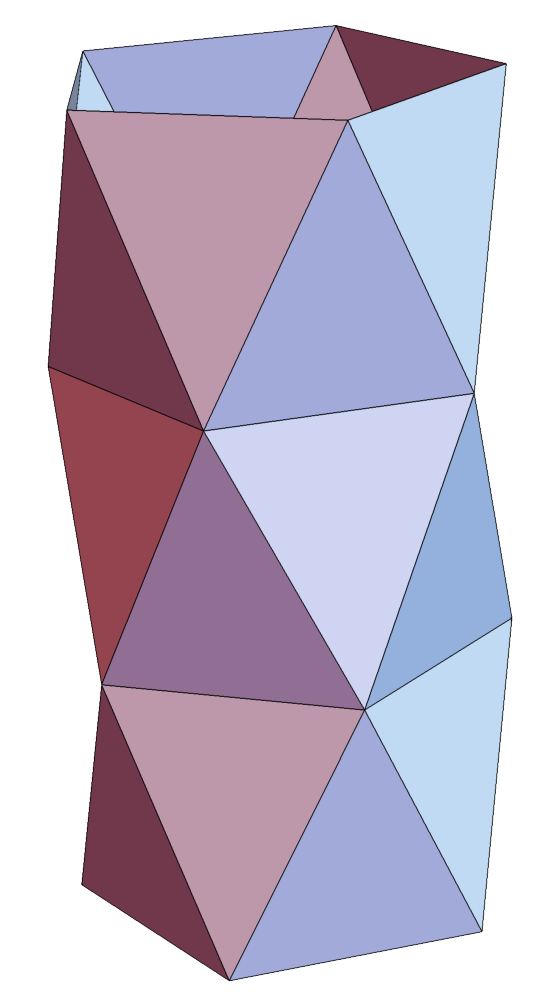
\includegraphics[width=1\textwidth]{uniform}
        \end{column}
    \end{columns}
\end{frame}

\begin{frame}
    \frametitle{Technicalities}
    Restrict to $1 + 1D$: curvature term is constant (Gau\ss -Bonnet) \\
    \begin{equation}
        S[T] \propto \text{Vol}(T) \propto N_2(T)
    \end{equation}
    After Wick rotation:
    \begin{equation}
        Z = \sum_{T} \frac{1}{C_T} e^{-\lambda N_2(T)}
    \end{equation}
    Label the triangles to simplify symmetry
    \begin{equation}
        Z_\ell = \sum _{T_\ell} \frac{1}{N_2(T_\ell)!} e^{-\lambda N_2(T)}
    \end{equation}
\end{frame}